\section{\textLR{STARK\cite{Stark}} \label{section:stark}}
\textRL{وهي اختصار لـ
\textLR{\textbf{s}patio-\textbf{t}emporal tr\textbf{a}nsfo\textbf{r}mer network for visual trac\textbf{k}ing}}،
في المقالة 
\textLR{\cite{Stark}}
 هناك نموذجان، النموذج الأول يستخدم فقط المعلومات المكانية لتحديد مكان الهدف، والنموذج الثاني هو بإضافة المعلومات الزمانية إلى النموذج الأول وذلك باستخدام 
\textLR{template}
\textRL{محدّث}
كدخل ثالث إلى النموذج. وهذه الطريقة لإدخال المعلومات الزمانية هي التي استخدمناها لتعديل خوارزمية 
\textLR{SwinTrack\cite{swinTrack}}.
\subsection{نموذج
\textLR{STARK}
الأول (مع المعلومات المكانية فقط)
}
البنية الأولية من خوارزمية 
 \textLR{STARK}
 والتي تستخدم فقط المعلومات المكانية موضحة في الشكل
 \ref{stark_base}،
 
 \begin{figure}[H]
\centerline{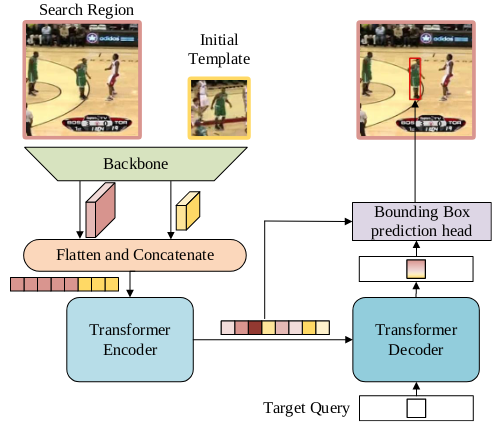
\includegraphics[scale=0.5]{images/stark_base}}
 	\caption{\textRL{
 			\textRL{مخطط النموذج الأول من خوارزمية}
 			\textLR{STARK}			
 	}}
 	\label{stark_base}
 \end{figure}
 \vspace{-8.0mm}
 \centerline{\textRL{
		\textRL{والذي يستخدم المعلومات المكانية فقط}
 		\textLR{\cite{Stark}}
 }}

%\begin{figure}[!h]
%	\centerline{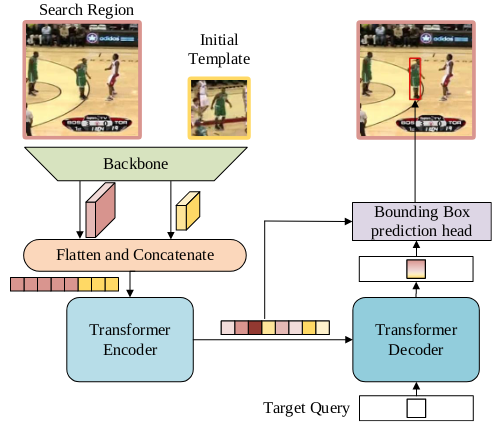
\includegraphics[scale=0.5]{images/stark_base}}
%	\caption{
%		\begin{footnotesize}
%		\textRL{مخطط النموذج الأول من خوارزمية}
%		\textLR{STARK}
%		\textRL{والذي يستخدم المعلومات المكانية فقط}
%		\textLR{\cite{Stark}}
%		\end{footnotesize}
%	}
%	\label{stark_base}	
%\end{figure}
للنموذج دخلان هما الـ
\textLR{template}
 من الإطار الأول لعملية الملاحقة 
$Z \in \Re^{{3} \mathsf{x} {H_z} \mathsf{x} W_z}$
حيث 
$H_z = W_z = 128$،
ونافذة البحث 
$X \in \Re^{{3} \mathsf{x} {H_x} \mathsf{x} W_x}$
حيث
$H_x = W_x = 320$.
\subsubsection{المرحلة الأولى - استخلاص السمات}
يتم استخلاص سمات كل من الدخلين عبر 
\textLR{backbone}،
 وهي المراحل الأربعة الأولى من شبكة
\textLR{ResNet\cite{ResNet}}،
فيكون
\textLR{stride}
 الشبكة 
 $s = 16$.
\newline
 خرج الـ
\textLR{backbone}
 هو سمات كل من الـ
\textLR{template}
$f_z \in \Re^{C \mathsf{x} \frac{H_z}{s} \mathsf{x} \frac{W_z}{s}}$،
وسمات نافذة البحث
$f_x \in \Re^{C \mathsf{x} \frac{H_x}{s} \mathsf{x} \frac{W_x}{s}}$.
بعدها  يتم سَلسَلة
\textLR{concatenate}
 سمات الـ
\textLR{template}
وسمات نافذة البحث ضمن سلسلة واحدة، ومن ثم تخفيض أبعاد السلسلة من 
\textLR{C}
إلى
\textLR{d}
، ثم تسطيح 
\textLR{flatten} 
 السلسلة لتصبح بأبعاد
$( d \mathsf{x} \frac{H_z}{s}\frac{W_z}{s} + \frac{H_x}{s}\frac{W_x}{s} )$،
وهذه السلسلة هي دخل المحول.
\subsubsection{المرحلة الثانية - المحول}
%تعتمد بنية المحول في هذه الخوارزمية بشكل كبير على محول  خوارزمية الكشف 
%\textLR{DETR\cite{DETR}}
%مع اختلافات طفيفة مثل عدد
%\textLR{target queries}.
يحتوي المرمز على $6$ طبقات، عدد الرؤوس في تابع الانتباه الذاتي متعدد الرؤوس
$ h=8 $,
أما أبعاد الطبقة المخفية  في شبكات 
\textLR{MLP}
فهي
 $2048$،
الترميز المكاني هو 
\textLR{sinusoidal}
كما في المحول الأصلي.
\newline
هدف  المرمز هو تعديل السمات بحسب السياق وإرسالها إلى مفكك الترميز.
من الشكل
\ref{stark_base}
نلاحظ دخلين لمفكك الترميز
الأول هو خرج المرمز، أما الثاني فهو
\textLR{target query}.
إن بنية المحول في
\textLR{STARK}
تعتمد بشكل كبير على المحول المستخدم في كاشف
\textLR{DETR\cite{DETR}}،
حيث عدد
\textLR{target queries}
هي عدد الأغراض التي يجب الكشف عنها. هنا في 
\textLR{STARK}
كخوارزمية ملاحقة لغرض واحد فإن عدد 
\textLR{target queries = 1}.
 \subsubsection{المرحلة الثالثة - تقدير مكان الهدف }
لتقدير المستطيل المحيط  بالغرض اعتمدت 
\textLR{STARK}
على الكتلة الموضحة في الشكل 
\ref{stark_score_head}
\begin{figure}[!h]
	\centerline{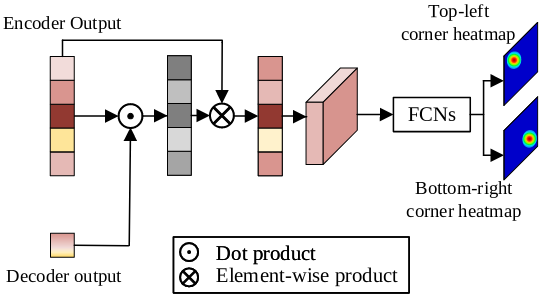
\includegraphics[scale=0.5]{images/stark_score_head}}
	\caption{
		\textRL{شبكة الـ}
		\textLR{regression}
		\textRL{لتقدير مكان الغرض}
		\textLR{\cite{Stark}}}
	\label{stark_score_head}
\end{figure}
هدف هذه الشبكة هو الـ
\textLR{regression}
، أي تقدير إحداثيات  الزاوية العليا اليسارية و الزاوية السفلى اليمينية للمستطيل المحيط.
بداية يحسب التشابه بين خرج المرمز وخرج مفكك الترميز،
 وذلك بحساب الجداء السلمي بينهما. نعدل خرج المرمز بتوزينه بقيم التشابه المحسوب سابقاً، نعدل من شكل خريطة السمات لتصبح ب
 $3$
  أبعاد 
$f \in \Re^{d \mathsf{x} \frac{H_s}{s} \mathsf{x} \frac{W_s}{s}}$.
ونقوم بإدخال خريطة السمات إلى شبكة 
\textLR{FCN}
 مكونة من $ 5$ طبقات تلاففية
\textLR{Conv-BN-ReLU}
 مع تابع تفعيل 
\textLR{ReLU}.
والخرج عبارة عن خريطة احتمالية لزوايا المستطيل المحيط.
\subsubsection{تابع الخطأ}
تابع الخطأ المستخدم في التدريب هو مجموع موزن لتابعين، الأول هو تابع الخطأ 
$L_1$،
والثاني هو
\textLR{GIOU\cite{giou}}
بحسب المعادلة التالية :
\begin{equation}
L = \lambda_{giou} L_{giou}(b_i,\hat{b}_i) + \lambda_{L_1} L_1(b_i,\hat{b}_i)
\label{loss_regression}
\end{equation} 
حيث 
$b_i$
هي القيمة الحقيقية 
\textLR{ground truth}
للمستطيل المحيط، بينما
$\hat{b}_i$
هي القيمة المقدرة (خرج الملاحق)، 
$\lambda_{giou},\lambda_l$
هي
\textLR{hyperparameters}.
\subsection{نموذج 
\textLR{STARK}
الثاني - مع المعلومات المكانية والزمانية}
معظم الملاحقات الحديثة تعتمد فقط على المعلومات المكانية أي معلومات مظهر الهدف وتتجاهل المعلومات الزمنية
\textLR{\cite{swinTrack},\cite{SiamFC}}.
حاولت خوارزمية
\textLR{STARK} 
إدخال المعلومات الزمانية عن طريق دخل ثالث وهو صورة الهدف في آخر عملية ملاحقة، وندعوه بالـ 
\textLR{dynamic template}.
هذا الـ
\textLR{template}
 الجديد الذي يحوي معلومات تغير مظهر الهدف هو ما نعتبره يحمل المعلومات الزمانية، بالإضافة إلى احتفاظ النموذج بالـ
\textLR{template}
الابتدائي.
\newline
يوضح الشكل 
\ref{stark-full}
النسخة الثانية 
(اللون الأحمر) على النسخة الأولية (اللون الأزرق) لخوارزمية 
\textLR{STARK}.
\begin{figure}[!h]
	\centerline{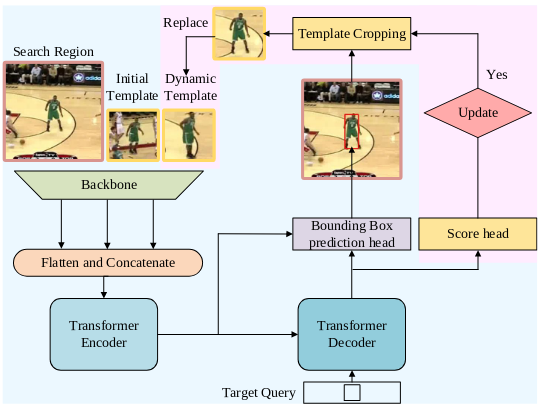
\includegraphics[width=\textwidth]{images/stark_full}}
	\caption{
		\textRL{النسخة الثانية من محول}
		\textLR{STARK}
		\textRL{باستخدام المعلومات الزمانية والمكانية}
		\textLR{\cite{Stark}}}
\label{stark-full}
\end{figure}
وكما في النموذج الأول يتم استخلاص سمات الـ
\textLR{template}
الجديد عبر
\textLR{backbone}،
و تكون مهمة المرمز هي استخلاص السمات المكانية والزمانية من شعاع سمات
 المداخل الثلاثة بعد سَلسَلتها.
\newline
التعديل الثاني في الخوارزمية هو معيار تحديث الهدف،
تم استخدام شبكة
\textLR{score head}
 غرضها التصنيف (هدف أو خلفية)،
% خرجها ندعوه بـ
%\textLR{score}،
يعبر خرجها
(\textLR{score})
 عن احتمالية وجود هدف في الموقع المقابل.
تحتوي الشبكة على ثلاث طبقات
\textLR{MLP}
%نسميها 
%\textLR{score head}،
بُعد الطبقة المخفية $256$، مع تابع تفعيل 
\textLR{sigmoid}.
\newline	
يتم تدريبها بتابع
\textLR{BCE binary cross-entropy}،
بحيث يكون خرج الشبكة
%(\textLR{score})
قيمة عالية عندما تكون وثوقية الهدف أكبر، 
\textRL{ولا يتم التحديث إلا }
عندما تكون هذه القيمة أكبر من حد معين
\textLR{threshold}،
تكون الوثوقية عالية طالما أن نافذة البحث تحوي كامل الهدف.
\newline
لتسهيل عملية تدريب النموذج الكلي
يتم تدريب النموذج على مرحلتين،
المرحلة الأولى يتم تدريب الشبكة بالكامل ماعدا شبكة التصنيف،
%\textLR{score head}،
أي باستخدام تابع الخطأ في المعادلة
\ref{loss_regression}.
المرحلة الثانية هي بتجميد أوزان المرحلة السابقة، وتدريب شبكة التصنيف
%\textLR{score head}
فقط، وذلك باستخدام تابع خطأ
\textLR{BCE}
كما في المعادلة
\ref{BCE}
\begin{equation}
	L_{ce} = log(P_i) + (1-y_i)log(1-P_i)
	\label{BCE}
\end{equation}
حيث
$y_i$
هي القيمة الحقيقة
\textLR{ground truth}،
$Pi$
هي خرج شبكة التصنيف.
\newline
أثناء التدريب يتم اختيار الـ
\textLR{template}
\textRL{الابتدائي}،
الـ
\textLR{template}
الديناميكي
\textRL{ ونافذة البحث}
بشكل عشوائي من
\textRL{القيم الحقيقية}
لمعطيات التدريب
\textRL{لنفس الفيديو}،
بحيث لا يكون البعد بينهما (عدد الإطارات) أكبر من قيمة ندعوها بـ
\textLR{update interval}.
طريقة التدريب هذه استعنّا بها عند تدريب النموذج الخاص بالبحث.
\newline
في مرحلة الملاحقة يتم تحديث الـ
\textLR{template}
 الديناميكي فقط عندما يكون عدد الإطارات بعد آخر تحديث أكبر من  
\textLR{update interval = 200}،
ويكون
$score > 0.5$.
\newline
يبين الجدول 
\ref{table:two_tracker_got10k_results}
نتائج التدريب على مجموعة المعطيات
\textLR{got10k}،
حيث
\textLR{STARK-S50}
 هي النسخة الأولى من الخوارزمية باستخدام المعلومات المكانية فقط، أي دون الـ
\textLR{template}
 الديناميكي، وباستخدام 
\textLR{ResNet50}
 كـ
\textLR{Backbone}.
\newline
\textLR{STARK-ST101}
 هي النسخة الثانية من الخوارزمية، أي باستخدام المعلومات المكانية والزمانية، وباستخدام
\textLR{ResNet101}
 كـ
\textLR{backbone}.
\newline
%****
البنية الصلبة المستخدمة في تدريب واختبار كلا النموذجين هي
\textLR{8 X 16GB Tesla V100 GPU}.
\newline
\textRL{
من الجدول 
\ref{table:two_tracker_got10k_results}
نلاحظ تحسن أداء خوارزمية 
\textLR{STARK}
عند إضافة الـ
\textLR{template}
المحدّث دون 
}
\textRL{
التأثير على سرعة الأداء، مع زيادة طفيفة في حجم النموذج في حال استخدام نفس الـ 
\textLR{backbone}.
}
% \selectlanguage{english}
%\begin{figure}[H]
%	\centering
%	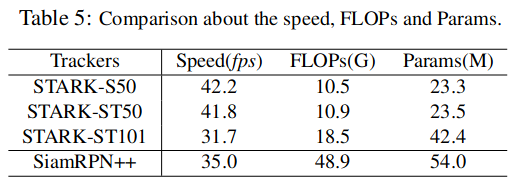
\includegraphics[width=\textwidth]{images/stark_speed}
%	\caption{
%		\cite{Stark}
%		speed of stark
%	}
%\end{figure}
%\selectlanguage{arabic}